\documentclass{article}
\usepackage[a4paper, total={170mm,257mm},margin=25mm]{geometry}

% Packages

\usepackage[utf8]{inputenc}
\usepackage{blindtext}
\usepackage[hidelinks]{hyperref}
\usepackage{amsmath }
\usepackage{siunitx}
\usepackage[acronym,toc,numberline]{glossaries}              % use glossaries-package 
\usepackage{xcolor}
\usepackage[parfill]{parskip}
\usepackage{minted}

\usepackage{graphicx}
\graphicspath{ {./Images/} }
\usepackage{subcaption}
\usepackage[export]{adjustbox}
\usepackage{multirow}

% For Code formatting

\usepackage{xcolor} % to access the named colour LightGray
\definecolor{LightGray}{gray}{0.9}
\definecolor{LightBlue}{rgb}{0.78, 0.9, 1.}
\usemintedstyle{ansimagenta}


\usepackage{stackengine}
% Package adjustment

\hypersetup{
    colorlinks,
    citecolor=black,
    filecolor=black,
    linkcolor=black,
    urlcolor=black
}



\newcommand{\rf}[1]{\textcolor{red}{#1}}
\newcommand{\sie}[1]{\text{\gls{symb:cameraMtx:#1}}}   %Symbol in equation
\newcommand{\sba}[1]{\gls{symb:cameraMtx:#1}}          % Symbol in text

\newcommand{\imgsec}[1]{
    \graphicspath{ {./Images/#1/} }
}
\newcommand{\imgsubsec}[2]{
    \graphicspath{ {./Images/#1/#2/} }
}

\newcommand{\degrs}{\ensuremath{^{\circ}}}

\newcommand\xrowht[2][0]{\addstackgap[.5\dimexpr#2\relax]{\vphantom{#1}}}

\newcommand{\symbsec}[1]{
    \renewcommand{\sie}[1]{\text{\gls{symb:#1:##1}}}
    \renewcommand{\sba}[1]{\gls{symb:#1:##1}}
}



\newcommand{\mlCode}[1]{
    \inputminted
    [
    breaklines=true,
    frame=lines,
    framesep=2mm,
    baselinestretch=1.2,
    bgcolor=LightBlue,
    fontsize=\footnotesize,
    linenos
    ]
    {matlab}{matlabFiles/#1}
}

\newcommand{\pyCode}[1]{
    \inputminted
    [
    breaklines=true,
    breakafter={,} ,
    frame=lines,
    framesep=2mm,
    baselinestretch=1.2,
    bgcolor=LightGray,
    fontsize=\footnotesize,
    linenos
    ]
    {python}{PythonFiles/#1}
}


\setlength{\glsdescwidth}{15cm}

\newglossary[slg]{symbolslist}{syi}{syg}{Symbolslist} % create add. symbolslist
\glsaddkey{unit}{\glsentrytext{\glslabel}}{\glsentryunit}{\GLsentryunit}{\glsunit}{\Glsunit}{\GLSunit}
\glsaddkey{eqtn}{\glsentrytext{\glslabel}}{\glsentryeqn}{\GLsentryeqn}{\glseqn}{\Glseqn}{\GLSeqn}


% -------------------------------------------------------------------
%                   Camera Matrix
% -------------------------------------------------------------------

\newglossaryentry{symb:cameraMtx:K}{name=$K$,
        description={Intrinsic Matrix of a pinhole camera model},
        unit={},
        eqtn={\ref{eq:Mtrx:Comb}, \ref{eq:Mtrx:Int}},
        type=symbolslist}
        
\newglossaryentry{symb:cameraMtx:P}{name=$P$,
        description={Pinhole Camera Matrix},
        unit={},
        eqtn={\ref{eq:Mtrx:Comb}},
        type=symbolslist}
        
\newglossaryentry{symb:cameraMtx:s}{name=$s$,
        description={Axis skew},
        unit={},
        eqtn={\ref{eq:Mtrx:Int}},
        type=symbolslist}
        
\newglossaryentry{symb:cameraMtx:f}{name=$f$,
        description={Focal Length},
        unit={pixels},
        eqtn={\ref{eq:Mtrx:Int}},
        type=symbolslist}
        
\newglossaryentry{symb:cameraMtx:eta}{name=$\eta$,
        description={Pixel skew},
        unit={},
        eqtn={\ref{eq:Mtrx:Int}},
        type=symbolslist}
        
\newglossaryentry{symb:cameraMtx:o_x}{name=$o_x$,
        description={Principle-point offset of the camera along the x-axis},
        unit={pixels},
        eqtn={\ref{eq:Mtrx:Int}},
        type=symbolslist}
        
\newglossaryentry{symb:cameraMtx:o_y}{name=$o_y$,
        description={Principle-point offset of the camera along the y-axis},
        unit={pixels},
        eqtn={\ref{eq:Mtrx:Int}},
        type=symbolslist}
        
\newglossaryentry{symb:cameraMtx:R}{name=$R$,
        description={Camera Rotation Matrix},
        unit={},
        eqtn={\ref{eq:Mtrx:Comb}, \ref{eq:Mtrx:Ext}},
        type=symbolslist}
        
\newglossaryentry{symb:cameraMtx:bt}{name=$\boldsymbol{t}$,
        description={Camera translation Matrix},
        unit={},
        eqtn={\ref{eq:Mtrx:Comb}, \ref{eq:Mtrx:Ext}},
        type=symbolslist}
        
\newglossaryentry{symb:cameraMtx:base}{name=$\boldsymbol{Baseline}$,
        description={Baseline between the cameras},
        unit={},
        eqtn={},
        type=symbolslist}

\newglossaryentry{symb:cameraMtx:F}{name=$F$,
        description={Focal length of the camera},
        unit={\si{mm}},
        eqtn={\ref{eq:Mtrx:fcl}},
        type=symbolslist}
        
\newglossaryentry{symb:cameraMtx:W_x}{name=$W_x$,
        description={Width of camera sensor},
        unit={\si{mm}},
        eqtn={\ref{eq:Mtrx:fcl}},
        type=symbolslist}
        
\newglossaryentry{symb:cameraMtx:w_x}{name=$w_x$,
        description={Width of camera sensor},
        unit={pixels},
        eqtn={\ref{eq:Mtrx:fcl}},
        type=symbolslist}
        
\newglossaryentry{symb:cameraMtx:kr}{name=$k_r$,
        description={Radial lens distortion coefficient},
        unit={pixels},
        eqtn={\ref{eq:Mtrx:rad}},
        type=symbolslist}


% -------------------------------------------------------------------
%                   Otsu thresholding
% -------------------------------------------------------------------


\newglossaryentry{symb:otsu:t}{name=$t$,
        description={Otsu threshold},
        unit={},
        eqtn={\ref{algo:otsu:main}},
        type=symbolslist}
        
\newglossaryentry{symb:otsu:sig}{name=$\sigma$,
        description={Variance (thresholding)},
        unit={},
        eqtn={\ref{algo:otsu:main}},
        type=symbolslist}
        
\newglossaryentry{symb:otsu:sig_bg}{name=$\sigma_{bg}$,
        description={Variance Background (thresholding)},
        unit={},
        eqtn={\ref{algo:otsu:main}},
        type=symbolslist}
        
\newglossaryentry{symb:otsu:sig_fg}{name=$\sigma_{fg}$,
        description={Variance Foreground (thresholding)},
        unit={},
        eqtn={\ref{algo:otsu:main}},
        type=symbolslist}
        
\newglossaryentry{symb:otsu:w_bg}{name=$\omega_{bg}$,
        description={Background thresholding weight},
        unit={},
        eqtn={\ref{algo:otsu:main}, \ref{algo:otsu:wts}},
        type=symbolslist}
        
\newglossaryentry{symb:otsu:w_fg}{name=$\omega_{fg}$,
        description={Foreground thresholding weight},
        unit={},
        eqtn={\ref{algo:otsu:main}, \ref{algo:otsu:wts}},
        type=symbolslist}
        
\newglossaryentry{symb:otsu:Pall}{name=$P_{all}$,
        description={Total number of pixels},
        unit={pixels},
        eqtn={\ref{algo:otsu:main}, \ref{algo:otsu:wts}},
        type=symbolslist}
        
\newglossaryentry{symb:otsu:Pfg}{name=$P_{FG}$,
        description={Total foreground pixels at threshold $t$},
        unit={pixels},
        eqtn={\ref{algo:otsu:main}, \ref{algo:otsu:wts}},
        type=symbolslist}
        
\newglossaryentry{symb:otsu:Pbg}{name=$P_{BG}$,
        description={Total background pixels at threshold $t$},
        unit={pixels},
        eqtn={\ref{algo:otsu:main}, \ref{algo:otsu:wts}},
        type=symbolslist}
        
\newglossaryentry{symb:otsu:xi}{name=$x_i$,
        description={Pixel $i$ value of the group},
        unit={},
        eqtn={\ref{algo:otsu:var}},
        type=symbolslist}
        
\newglossaryentry{symb:otsu:xb}{name=$\bar{x}$,
        description={Mean values of the group of pixels},
        unit={},
        eqtn={\ref{algo:otsu:var}},
        type=symbolslist}
        
\newglossaryentry{symb:otsu:N}{name=$N$,
        description={Number of pixels},
        unit={pixels},
        eqtn={\ref{algo:otsu:var}},
        type=symbolslist}
        
        
% -------------------------------------------------------------------
%                   Suzuki Contouring
% -------------------------------------------------------------------

\newglossaryentry{symb:suzuki_contour:N}{name=$N$,
        description={Number of pixels},
        unit={pixels},
        eqtn={\ref{algo:otsu:var}},
        type=symbolslist}
        
        
        
        
        
        
% -------------------------------------------------------------------
%                   Robotic Arm Design
% -------------------------------------------------------------------

\newglossaryentry{symb:rba:s0}{name=$S_0$,
        description={Link between the base and the first joint},
        unit={mm},
        eqtn={\ref{fig:arm:basestruct}},
        type=symbolslist}
        
\newglossaryentry{symb:rba:s1}{name=$S_1$,
        description={Link between the first and second joint},
        unit={mm},
        eqtn={\ref{fig:arm:basestruct}},
        type=symbolslist}
        
\newglossaryentry{symb:rba:s2}{name=$S_2$,
        description={Link between the second and the third joint},
        unit={mm},
        eqtn={\ref{fig:arm:basestruct}},
        type=symbolslist}
        
\newglossaryentry{symb:rba:s3}{name=$S_3$,
        description={Link between the third and fourth joint},
        unit={mm},
        eqtn={\ref{fig:arm:basestruct}},
        type=symbolslist}
        
\newglossaryentry{symb:rba:s4}{name=$S_4$,
        description={Link between the fourth and the last joint},
        unit={mm},
        eqtn={\ref{fig:arm:basestruct}},
        type=symbolslist}
        
\newglossaryentry{symb:rba:s5}{name=$S_5$,
        description={Link between the last joint and the cup connector.},
        unit={mm},
        eqtn={\ref{fig:arm:basestruct}},
        type=symbolslist}
        
\newglossaryentry{symb:rba:j0}{name=$J_0$,
        description={Thrust Rotation joint in the base of the arm.  The direction of rotation in relation to the previous connected link is $\theta_r$.},
        unit={},
        eqtn={\ref{fig:arm:basestruct}},
        type=symbolslist}
        
\newglossaryentry{symb:rba:j1}{name=$J_1$,
        description={Radial Rotation joint of the robotic arm.  he direction of rotation in relation to the previous connected link is $\varphi_r$.},
        unit={},
        eqtn={\ref{fig:arm:basestruct}},
        type=symbolslist}
        
\newglossaryentry{symb:rba:j2}{name=$J_2$,
        description={Radial Rotation joint of the robotic arm.  he direction of rotation in relation to the previous connected link is $\varphi_r$.},
        unit={},
        eqtn={\ref{fig:arm:basestruct}},
        type=symbolslist}
        
\newglossaryentry{symb:rba:j3}{name=$J_3$,
        description={Radial and thrust Rotation joint of the robotic arm.  The direction of rotation in relation to the previous connected link is $\theta_r$.},
        unit={},
        eqtn={\ref{fig:arm:basestruct}},
        type=symbolslist}
        
\newglossaryentry{symb:rba:j4}{name=$J_4$,
        description={Radial Rotation joint of the robotic arm.  he direction of rotation in relation to the previous connected link is $\varphi_r$.},
        unit={},
        eqtn={\ref{fig:arm:basestruct}},
        type=symbolslist}
        
\newglossaryentry{symb:rba:j5}{name=$J_5$,
        description={Radial rotation joint of the robotic arm.  The direction of rotation in relation to the previous connected link is $\theta_r$.},
        unit={},
        eqtn={\ref{fig:arm:basestruct}},
        type=symbolslist}
        
\newglossaryentry{symb:rba:thrust_r}{name=$\theta_r$,
        description={Rotational direction of a joint which keeps the angle between the connected links constant.},
        unit={deg},
        eqtn={\ref{fig:arm:basestruct}},
        type=symbolslist}
        
\newglossaryentry{symb:rba:radial_r}{name=$\varphi_r$,
        description={Rotational direction of a joint which changes the angle between the connected links.},
        unit={deg},
        eqtn={\ref{fig:arm:basestruct}},
        type=symbolslist}
        

% Point system

\newglossaryentry{symb:rba:porig}{name=$P_{ORIG}$,
        description={The point of the rotational centre of $J_1$ in three dimensional space, which is used as the origin point of the system.},
        unit={mm},
        eqtn={\ref{fig:arm:basestruct}},
        type=symbolslist}
        
\newglossaryentry{symb:rba:pcup}{name=$P_{cup}$,
        description={The point of the rotational centre of the cup in three dimensional space in relation to $P_{ORIG}$.},
        unit={mm},
        eqtn={\ref{fig:arm:basestruct}},
        type=symbolslist}

% --------------------------------------------------------
%                   Section headings for glossaries
% --------------------------------------------------------

% \newglossaryentry{otsu}
% {
%     name=Otsu threshold,
%     description={An adaptive thresholding technique}
% }

% \newglossaryentry{cameraMtx}
% {
%     name=Camera Matrix,
%     description={An adaptive thresholding technique}
% }


% --------------------------------------------------------
%                   Rest of glossaries
% --------------------------------------------------------

\newglossaryentry{GCD}
{
    name=Greatest Common Divisor,
    description={Is a markup language specially suited for 
scientific documents}
}

\newglossaryentry{TST}
{
    name=Test,
    description={Is a markup language specially suited for 
scientific documents}
}

\newglossaryentry{FOV}
{
    name=field of view,
    description={is the maximum field (often expressed as an angle) which the camera can capture of an environment.}
}

\newglossaryentry{RadDist}
{
    name=radial distortion,
    description={a non-linear camera distortion caused by the lens that causes straight lines to be captured as curved in images.}
}

\newacronym{gcd}{GCD}{\gls{GCD}}
\newacronym{fov}{FOV}{\gls{FOV}}
% \makeglossaries
\makenoidxglossaries


\title{Depth_Vision_Planning and Mapping}
\author{Matthieu Christofides}
\date{October 2021}


% Document

\begin{document}

% \maketitle
\newpage

\tableofcontents

\section{Calibration}

Binary depth vision is calculated by comparing two images which are placed a specified distance (\sba{base}) from eachother.  The distance of each object is calculated by finding the difference between points in each camera.  This comparison can however not be made with raw camera feeds due to the difference in manufacturing and digitizing of each camera sensor.  To correct the distortion, difference in focal lengths, rotation and translation of the camera sensors, the cameras require calibration.\\

Each camera could have different distortions, focal lengths and world positions.  The parameters of each camera and the cameras in relation to each other can be found by determining the intrinsic (\sba{K}) and extrinsic parameters of each camera.



\  \\

\subsection{Camera Model} \label{sec:cameraMtx}
\symbsec{cameraMtx}

A camera is modeled after the Pin hole camera model (\sba{P}) proposed by \rf{ref}.  The camera model (equation \ref{eq:Mtrx:Comb}) consists of the intrinsic camera matrix (\sba{K}) and the extrinsic camera matrix.  \sba{P} represents the coordinates in the image.

\begin{align}
\begin{split}\label{eq:Mtrx:Comb}
    \sie{P} &= \overbrace{\sie{K}}^{\text {Intrinsic Matrix }} \times \overbrace{[\sie{R} \mid \sie{bt}]}^{\text {Extrinsic Matrix }} \\
    \text{Where,}& \\
    \sie{P} &= \left[\begin{array}{l}
x \\
y \\
1
\end{array}\right]
\end{split}
\end{align}

\subsubsection{Intrinsic camera Matrix (\sba{K})}

The intrinsic camera matrix (equation \ref{eq:Mtrx:Int})(\href{robots.ox.ac.uk/~vgg/hzbook/}{Hartley and Zisserman}) defines the unique characteristics of each camera.  The matrix consists of the focal lengths, axis skew, and principle-point offsets.

\begin{align}
    \sie{K} &= \left[\begin{array}{ccc}
    \sie{f} & \sie{s} & \sie{o_x} \\
    0 & \sie{eta}\sie{f} & \sie{o_y} \\
    0 & 0 & 1
    \end{array}\right] \label{eq:Mtrx:Int}
\end{align}

The axis skew (\sba{s}) represents the angle between the x-axis and y-axis of the image.  In most current digital cameras axis skew is either zero or negligible, however during the digitisation of the analogue images, a non-zero axis skew can be introduced when the pixels are not vertically synchronized during frame capturing process. \href{http://epixea.com/research/multi-view-coding-thesisch2.html#x13-320002.2.1}{\rf{Source}}.

The optical centre of the sensor to the lens may not be in the centre of the image.  The principle-offset of the optical centre from the centre of the image is represented in the x-axis by \sba{o_x} and in the y-axis by \sba{o_y}.

The focal length (\sba{f}) is measured in pixels and represents the focal length of the camera, which is the distance between the image plane and the optical centre \rf{Include an image}.  It does however happen that the pixels themselves could be skewed, in which case the focal length in the x and y-axis would differ.  The angle of this pixel skew is represented by \sba{eta} and is initially assumed to be \sba{eta}=1.  The focal length can be converted from pixels to mm by equation \ref{eq:Mtrx:fcl}.

\begin{align}
    \sie{F} &= \sie{f}\frac{\sie{W_x}}{\sie{w_x}} \label{eq:Mtrx:fcl}
\end{align}

\subsubsection{Radial Distortion}

The internal matrix of a camera is however not the only parameters required to \rf{rectify} an image as there are non-linear distortions also present from the parameters of the lenses used.  There are different causes of distortion with different results, eg. radial distortion caused by the lens bending to provide the desired \acrlong{fov} (\acrshort{fov}), planar (tangential) distortion which is an effect of lens misalignment to the camera sensor and distortions caused by imperfections in the lens.

This project will only be discussing Radial Distortion effects and corrections of the non-linear distortions.  \Gls{RadDist} is when a straight line in the world is captured as a curved line in the image.  These can most commonly be found in wide angle cameras lenses, which cause barrel distortion \rf{Add image} as the image magnification decreases from the principle point of the camera.  Pincushion distortion (\rf{add image}) is the opposite of barrel distortion, and is caused by telephoto lenses mostly.

Radial distortion is dependent on the location of the pixel from the principle point of the image.  This non-linear distortion can be estimated by finding the radial distortion coefficient (\sba{kr}) in equation \ref{eq:Mtrx:rad}.

\begin{align}
    \begin{split}
        x_c &= x(1+\sie{kr}r^2)\\
        y_c &= y(1+\sie{kr}r^2) \label{eq:Mtrx:rad}
    \end{split}
\end{align}

\rf{How to find $k_r$}

\subsubsection{Tangential distortion}

\rf{New sensors may need tangential distortion correction}


\subsubsection{Extrinsic camera Matrix}

The extrinsic camera matrix relates 

\begin{align}
[\sie{R} \mid \sie{bt}] &=\left[\begin{array}{ccc|c}
r_{11} & r_{12} & r_{13} & t_{1} \\
r_{21} & r_{22} & r_{23} & t_{2} \\
r_{31} & r_{32} & r_{33} & t_{3}
\end{array}\right] \label{eq:Mtrx:Ext}
\end{align}


Equation \ref{eq:Mtrx:Comb} can thus be expanded to equation \ref{eq:Mtrx:CombFull}.

\begin{align}
\left[\begin{array}{l}
x \\
y \\
1
\end{array}\right]=\left[\begin{array}{ccc}
    \sie{f} & \sie{s} & \sie{o_x} \\
    0 & \sie{eta}\sie{f} & \sie{o_y} \\
    0 & 0 & 1
    \end{array}\right]\left[\begin{array}{cccc}
r_{11} & r_{12} & r_{13} & t_{1} \\
r_{21} & r_{22} & r_{23} & t_{2} \\
r_{31} & r_{32} & r_{33} & t_{3}
\end{array}\right]\left[\begin{array}{c}
X \\
Y \\
Z \\
1
\end{array}\right] \label{eq:Mtrx:CombFull}
\end{align}


Intrinsic camera pin hole model intrinsic matrix

% \textbf{Links Tsai Calibration:}
% \begin{itemize}
%     \item \href{https://en.wikipedia.org/wiki/Camera_resectioning#Tsai.27s_Algorithm}{Wikipedia Tsai Basic}
%     \item \href{https://en.wikipedia.org/wiki/Pinhole_camera_model}{Pinhole Camera Model (Wiki)}
%     \item \href{https://github.com/bailus/tsai-calibration}{Github Impl 1}
%     \item \href{https://github.com/siddharthKatageri/tsai-camera-calibration}{Github impl 2}
% \end{itemize}
% \textbf{Links Camera Models:}
% \begin{itemize}
%     \item \href{https://ksimek.github.io/2013/08/13/intrinsic/}{Pinhole model}
%     \item \href{https://ksimek.github.io/perspective_camera_toy.html}{Pinhole camera Toy}
% \end{itemize}

% \subsection{Tsai vs Zhang}

% \textbf{\textit{Algos:}}
% \begin{itemize}
%     \item HSV Filtering
%     \item Otsu Threshold - \href{https://muthu.co/otsus-method-for-image-thresholding-explained-and-implemented/}{Math}
%     \item Median Blur
%     \item Suzuki contouring - \href{https://theailearner.com/tag/suzuki-contour-algorithm-opencv/}{Math}
%     \item Harris Corner detection - \href{https://muthu.co/harris-corner-detector-implementation-in-python/}{Math}
% \end{itemize}

% \acrlong{gcd}


% \glsaddall[types={symbolslist}]



% \textbf{Variables explained}
% \end{equation}


\subsection{Algorithms}

% Best Explenation
% https://muthu.co/otsus-method-for-image-thresholding-explained-and-implemented/
\subsubsection{Otsu Thresholding} \label{sec:otsu}
\symbsec{otsu}

\rf{Different thresholding methods}

Thresholding is the process of separating desired pixels or information from the rest of the image.  Otsu's variance-based thresholding iterates through a set of thresholding values to minimise the spread of background and foreground pixels in a gray scale image.  The weighted variance between the background and foreground pixels are represented by \sba{w_bg} and \sba{w_fg} respectively as functions of the threshold (\sba{t}) in equation \ref{algo:otsu:main}.

\begin{align}
    \sie{sig}^{2}(\sie{t}) &= \sie{w_bg}(\sie{t}) \sie{sig_bg}^{2}(\sie{t})+\sie{w_fg}(\sie{t}) \sie{sig_fg}^{2}(\sie{t}) \label{algo:otsu:main}
\end{align}

The weights used to calculate the variance can by determined by equation \ref{algo:otsu:wts}.  \sba{Pall} represents the total number of pixels in the image.  \sba{Pbg} and \sba{Pfg} is the background and foreground number of pixels based on the threshold that is being tested.

\begin{align}
    \begin{split}
        \sie{w_bg}(\sie{t}) &=\frac{\sie{Pbg}(\sie{t})}{\sie{Pall}} \\
        \sie{w_fg}(\sie{t}) &=\frac{\sie{Pfg}(\sie{t})}{\sie{Pall}} 
    \end{split}\label{algo:otsu:wts}
\end{align}

The variance is calculated then by summing the square of the difference between the value of each pixel (\sba{xi}) and the mean value of the pixels (\sba{xb}).  The sum is then divided by the total number of pixels in the group (\sba{N}) minus 1.  Equation \ref{algo:otsu:var} is thus used to calculate both \sba{sig_bg} and \sba{sig_fg} at the current threshold.  After all of these values have been found equation \ref{algo:otsu:main} is then used to calculate the total variance at the current threshold.

\begin{align}
    \sie{sig}^{2}(\sie{t})&=\frac{\sum\left(\sie{xi}-\sie{xb}\right)^{2}}{\sie{N}-1} \label{algo:otsu:var}
\end{align}

% Best Explenation 
% https://theailearner.com/tag/suzuki-contour-algorithm-opencv/
\subsubsection{Suzuki’s Contour tracing algorithm}
\symbsec{suzuki_contour}

\rf{Remember to illustrate}


\subsection{Harrison Corner Detection}

\rf{Insert example image}

The detection of the calibration points of the checkered board requires an accurate location of the checkered board intersections in the image and relate it to the real world points.  When using the Tsai camera calibration not many points nor images are required for the calibration, and can thus be accomplished by hand.  When using the Zhang camera calibration, multiple points and images are required for accurate calibration.

The most common detector used for this type of corner detection, is the Harris corner detection \rf{ref}\rf{slidesref}.  The detection of the corners are based on the autocorrelation function in equation \ref{algo:harris:main}.  The function makes use of a sliding window ($w(x, y)$) to compare neighbouring intensities and find interest points.  The window can either be a rectangular window, or a pixel-weighted Gaussian window.  The difference between the shifted intensity and the current window intensity is then determined to find the interest points.

\begin{align}
    E(u, v)=\sum_{x, y} \underbrace{w(x, y)}_{\text {window function }}[\underbrace{I(x+u, y+v)}_{\text {shifted intensity }}-\underbrace{I(x, y)}_{\text {intensity }}]^{2} \label{algo:harris:main}
\end{align}

The shifted intensity can be simplified by using the first-order Taylor expansion which simplifies equation \ref{algo:harris:main} to equation \ref{algo:harris:taylr1}.  The covariance ($M$) is then used to determine the function of the ellipse at $u,v$.  

\begin{align}
    \begin{split} \label{algo:harris:taylr1}
         E(u, v) &\approx\left[\begin{array}{ll}u & v\end{array}\right] M\left[\begin{array}{l}u\\v\end{array}\right]\\
        M&=\sum_{x, y} w(x, y)\left[\begin{array}{ll}I_{x} I_{x} & I_{x} I_{y} \\I_{x} I_{y} & I_{y} I_{y}\end{array}\right]
    \end{split}
\end{align}

To calculate the harris response ($R$), the eigenvalues of the covariance ($\lambda_1$ and $\lambda_2$) is required \rf{Insert image}.  \rf{Expand on lambdas for corner, edge and flat regions}.  The mathematical expression of the harris response can be defined in terms of the eigenvalues of the covariance matrix, as shown in equation \ref{algo:harris:rspE}.  As the determinant of the covariance matrix is the same as the product of the eigenvalues of the matrix, and the trace of the covariance matrix is the same as the sum of the eigenvalues, the equation can be simplified to equation \ref{algo:harris:rspF}.  \rf{Mention Triggs and Szeliski versions, why was Szeliski used maybe?}

\begin{align}
    R &= \lambda_1\lambda_2 - k (\lambda_1 + \lambda_2)^2 \label{algo:harris:rspE}\\
    R &= det(M) - k(traceM)^2 \label{algo:harris:rspF}
\end{align}

To determine corners, edges and flat regions of the image, the following can be applied:

\begin{align*}
    \text{Flat regions:   } R &\approx 0\\
    \text{Corners:   } R &>0 \\
    \text{Edges:   } R &< 0
\end{align*}


\rf{This is part of implementation, not design}
The spatial derivatives in the vertical and horizontal directions can be approximated by using the Sobel operator \rf{ref}.  The Sobel operator convolves two 3x3 kernels with the gray-scale image to accentuate the edges of objects in the image based on the gradient changes.  These gradient changes are filtered for in both the x- and y-axis.  $G_x$ is the x-axis kernel, and $G_y$ the y-axis kernel (equation \ref{algo:sobel}).

% This image can also be threshold by an algorithm like the Otsu thresholding or adaptive thresholding to filter out noise, adjust the gamma of an image, blurring the image, 

\begin{align}
    \begin{split} \label{algo:sobel}
    G_x&=\left[\begin{array}{lll}
        +1 & 0 & -1 \\
        +2 & 0 & -2 \\
        +1 & 0 & -1
        \end{array}\right] * \mathbf{A} \quad \\
    \quad G_y&=\left[\begin{array}{ccc}
        +1 & +2 & +1 \\
        0 & 0 & 0 \\
        -1 & -2 & -1
        \end{array}\right] * \mathbf{A}
    \end{split}
\end{align}

\rf{Excellent explanation: \href{https://www.youtube.com/watch?v=_qgKQGsuKeQ&t=2545s}{Youtube lecture}}

\subsection{Saddle Point detection}



\subsection{Coordinate to real world points}

\rf{Compare Tsai results, and maybe include source in appendix if space... my time spent does not mean include!}


\subsection{Direct Linear Transform (DLT)}


\subsection{Zhang implementation}

Zhang uses planar calibration Matrix

As shown in equations \ref{eq:Mtrx:Comb} and \ref{eq:Mtrx:CombFull}, the camera matrix is calculated by finding the intrinsic and extrinsic parameters.  As Zhang's camera calibration method uses only a planar calibration checkered board, the $Z$ coordinate of the world points can be disregarded as it stays constant if the plane is assumed to be the origin.  This thus allows us to simplify equation \ref{eq:Mtrx:CombFull} to equation \ref{algo:zhang:fund}.

\symbsec{cameraMtx}
\begin{align}
\left[\begin{array}{l}
x \\
y \\
1
\end{array}\right]=\left[\begin{array}{ccc}
    \sie{f} & \sie{s} & \sie{o_x} \\
    0 & \sie{eta}\sie{f} & \sie{o_y} \\
    0 & 0 & 1
    \end{array}\right]\left[\begin{array}{ccc}
r_{11} & r_{12} & t_{1} \\
r_{21} & r_{22} & t_{2} \\
r_{31} & r_{32} & t_{3}
\end{array}\right]\left[\begin{array}{c}
X \\
Y \\
1
\end{array}\right] \label{algo:zhang:fund}
\end{align}

When the world points and image points are replaced into equation \ref{algo:zhang:fund}, equation \ref{algo:zhang:perPnt} is found.

\begin{align}
\left[\begin{array}{c}
x_{i} \\
y_{i} \\
1
\end{array}\right]=\underset{3 \times 3}{H}\left[\begin{array}{c}
X_{i} \\
Y_{i} \\
1
\end{array}\right] \quad i=1, \ldots, I \label{algo:zhang:perPnt} 
\end{align}

\subsection{8-point Algorithm}

% More than 8 points, matrix becomes regular but should not.

Two sets of points and intrinsic matrices
\begin{itemize}
    \item Left camera: $p_l$ and $K_l$
    \item Right camera: $p_r$ and $K_r$
\end{itemize}

Normalize points $p_l$ and $p_r$ and denote as $p_{ln}$ and $p_{rn}$

$A$ is then calculated for each homologous (\rf{means corresponding point in each image}) set of points of $p_{ln}$ and $p_{rn}$ with equation \ref{algo:A}.  $i$ is the current point, $x_{ln}$ and $y_{ln}$ is the left and right components respectively.

\begin{align}
    A(i) &= [x_{rn}(i) \times  x_{ln}(i), x_{rn}(i) \times  y_{ln}(i), x_{rn}(i), y_{rn}(i) \times  x_{ln}(i), y_{rn}(i) \times  y_{ln}(i), y_{rn}(i), x_{ln}(i), y_{ln}(i), 1] \label{algo:A}
\end{align}

$N$ is the number of points

\begin{itemize}
    \item $A$ is a $Nx9$ Matrix
    \item $U$ is a $NxN$ Matrix
    \item $D$ is a $Nx9$ Matrix
    \item $V^T$ is a $9x9$ Matrix
\end{itemize}
 consist of the vectors $U$, $D$ and $V^T$.

\begin{align}
A=U D V^{T} \label{algo:8pnt:base}
\end{align}

Find the single value decomposition (SVD) of $A$


Need to enforce rank 2 on the fundamental Matrix:

Use $V^T$ to fill the temporary Fundamental matrix $F^{\top}$

\begin{align}
U D V^{\top} &= \text{SVD}(F^{\top})\label{algo:8pnt:base}
\end{align}

Find the new Fundamental Matrix then:
\begin{align}
    F &= U \operatorname{diag}\left(D_{11}, D_{22}, 0\right) V^{\top}
\end{align}

The normalisation is reversed on F then to obtain final fundamental Matrix.  The transpose of the intrinsic matrix $K_2$ is multiplied with the Fundamental matrix, which is multiplied with the intrinsic matrix of the first camera $K_1$

\begin{align}
    E &= K_2^{\top} \times F \times K_1
\end{align}

The rotation matrix ($R$) and translation matrix ($T$) of the right camera to the left, can be determined by equation \ref{algo:Edecomp}.

\begin{align}
E=\left[\begin{array}{ccc}
0 & -T_{2} & T_{1} \\
T_{2} & 0 & -T_{0} \\
-T_{1} & T_{0} & 0
\end{array}\right] R \label{algo:Edecomp}
\end{align}

The baseline of the cameras can be determined from the translation matrix.  These matrices will also show the vertical, horizontal and rotational differences between the two cameras.

These Extrinsic parameters can then be used to align the camera images after they have been rectified.

\rf{This comes under the results section}

While the rotation matrix $R$ should ideally be a 3x3 identity matrix, the difference show the slight deviations during manufacturing.  The translation matrix ($T$) is ideally the Baseline distance and 0,0.  This is however also slightly different due to manufacturing not being perfect.





% A = UDV^T



\subsection{Extrinsic parameter implementation}

Summary
\begin{itemize}
    \item Relative orientation (rotation and translation matrix)
    \item Fundamental Matrix
    \item Essential Matrix
\end{itemize}

(total 12 parameters)

\section{Depth Tracking}

\subsection{Camera Image rectification}
\subsection{Camera Image cropping and alignment}
\subsection{Disparity Mapping}
\subsection{Q Matrix for real depth Map}



\section{Facial Recognition}

\subsection{Viola-Jones}
\imgsubsec{FacialRecognition}{ViolaJones}

\subsubsection{Input Image Preprocessing}

\begin{enumerate}
    \item Gray scale of image
    \item calculate integral of image (show integral image calculation)
\end{enumerate}

\subsubsection{Integral Image}

An integral image is calculated before hand by summing all values from the upper-left pixel to the current pixel.  This reduces calculation time for each rectangular window as instead of having to sum each value in the window, only four values have to be used to calculate the sum of all the values in a window.  Suppose the image values looks like shown in figure \ref{fig:vj:exm} with the integral of the image shown in figure \ref{fig:vj:int}.  Instead of summing each value in the blue square in figure \ref{fig:vj:exm} (as shown in equation \ref{eq:vj:exm}), the two orange values (19 and 15) in figure \ref{fig:vj:int} can be subtracted from the sum of the blue values (6 and 50) in figure \ref{fig:vj:int} to find the sum of the values in the window (shown in equation \ref{eq:vj:intS}).

\begin{figure}[h]
    \begin{subfigure}{0.5\textwidth}
        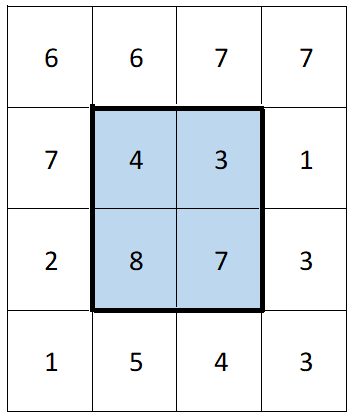
\includegraphics[width=0.9\linewidth, height=4.5cm,keepaspectratio,center]{exampleImg.png} 
        \caption{Image example}
        \label{fig:vj:exm}
    \end{subfigure}
    \begin{subfigure}{0.5\textwidth}
        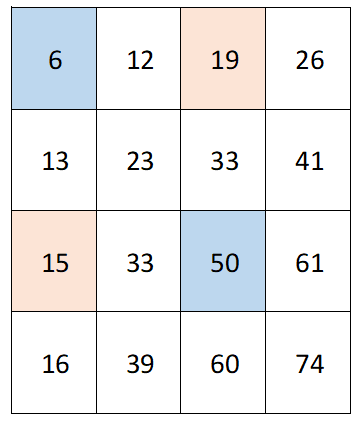
\includegraphics[width=0.9\linewidth, height=4.5cm,center,keepaspectratio]{IntegralImg.png}
        \caption{Integral Image}
        \label{fig:vj:int}
    \end{subfigure}
    \caption{Integral Image Calculations}
    \label{fig:vj:main}
\end{figure}

\begin{align}
    4 + 3 + 8 + 7 &= 22 \label{eq:vj:exm}\\
    50 + 6 - 15 - 19 &= 22 \label{eq:vj:intS}
\end{align}

  For a window of size 2x2 this adds to be the same number of calculations, thus adding no value.  However, if the window size is 255x255 of a 1280x720 image, the summation calculations require 65025 operations, while the integral image only takes four operations still.  As the sum of various size windows (for various size faces in the image) and multiple windows of each size (to scan the image) are calculate, this decrease in operations greatly increases the efficiency and speed of the calculations.

\subsubsection{Haar features}

The Haar features that are searched for look like in figure \ref{fig:vj:edgehaar}.  The white and black regions can be interchanged for white 'lines' instead of black 'lines' as well.

\begin{figure}[h]
    \begin{subfigure}{0.19\textwidth}
        
\includegraphics[width=0.9\linewidth, height=1.5cm,keepaspectratio,center]{edgeFeature_1.png} 
    \end{subfigure}
    \begin{subfigure}{0.19\textwidth}
        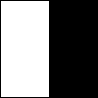
\includegraphics[width=0.9\linewidth, height=1.5cm,center,keepaspectratio]{edgeFeature_2.png}
    \end{subfigure}
    \begin{subfigure}{0.19\textwidth}
        
\includegraphics[width=0.9\linewidth, height=1.5cm,center,keepaspectratio]{lineFeature_1.png}
    \end{subfigure}
    \begin{subfigure}{0.19\textwidth}
        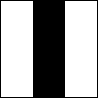
\includegraphics[width=0.9\linewidth, height=1.5cm,center,keepaspectratio]{lineFeature_2.png}
    \end{subfigure}
    \begin{subfigure}{0.19\textwidth}
        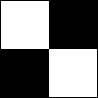
\includegraphics[width=0.9\linewidth, height=1.5cm,center,keepaspectratio]{chckFeature.png}
    \end{subfigure}
    \caption{Haar Features.}
    \label{fig:vj:edgehaar}
\end{figure}

\subsubsection{AdaBoost Training}

As there can be more than 180000 features in a 24x24 image \rf{ref}, the features that are not useful must be filtered out.  This is accomplished by using a dataset of facial images and non-facial images (images are categorised) to filter out the useful haar features ($f_n$ in equation \ref{eq:vj:adabst:main}) as well as their weights ($\alpha_{n}$ in equation \ref{eq:vj:adabst:main}) unique to faces.  Viola and Jones used 4960 faces and 9544 non-faces as training data for the algorithm.  As some of the features are found in both faces and non-faces, it is the combination of features that determines the algorithm's confidence of whether or not it is a face (equation \ref{eq:vj:adabst:main}). 

\begin{align}
    F(x)=\alpha_{1} f_{1}(x)+\alpha_{2} f_{2}(x)+\alpha_{3} f_{3}(x)+\ldots+\alpha_{n} f_{n}(x) \label{eq:vj:adabst:main}
\end{align}

Should a face be found in the image, the result ($y_n$) is equals 1, and if no face is found the result is returned as 0.  This is then compared to the known results of the faces and non-faces.  The weights are initialised by equation \ref{eq:vj:ada:wts:int}.  $N$ is the total number of images used for the training.

\begin{align}
    w_{1}^{i}=\frac{1}{N} \label{eq:vj:ada:wts:int}
\end{align}

The weights are then normalised (equation \ref{eq:vj:ada:wts:norm} with $w_t$ being the probability distribution for each classifier ($t$).  A single feature classifier ($f_t$) and evaluate the error of the classifier with respect to $w_t,i$ as shown in equation \ref{eq:vj:ada:wts:err}, and the classifier with the lowest error is selected.  

\begin{align}
    w_{t, i}&=\frac{w_{t, i}}{\sum_{j=1}^{N} w_{t, j}} \label{eq:vj:ada:wts:norm} \\
    \epsilon_{j}&=\sum_{i} w_{t, i}\left|f_{t}\left(x_{i}\right)-y_{i}\right| \label{eq:vj:ada:wts:err}
\end{align}

The weights are then updated by equation \ref{eq:vj:ada:wts:updt}.

\begin{align}
    \begin{split}
        w_{t+1, i}&=w_{t, i} \beta^{1-\epsilon_{t}}\\
        \beta_{t}&=\frac{\epsilon_{t}}{1-\epsilon_{t}}\\
        \alpha_{t}&=\log \left(\frac{1}{\beta_{t}}\right)
    \end{split}  \label{eq:vj:ada:wts:updt}
\end{align}

The final sum and weights of the haar classifiers can then be defined by equation \ref{eq:vj:ada:wts:final}.

\begin{align}
    F(x)=\left\{\begin{array}{c}
    1 \text { if } \sum_{t=1}^{T} \alpha_{t} f_{t}(x) \geq 0.5 \sum_{t=1}^{T} \alpha_{t} \\
    0 \text { otherwise }
    \end{array}\right. \label{eq:vj:ada:wts:final}
\end{align}

Calculating all of the features, multiplying their weights and summing the results for each window in the image can decrease the speed of the calculations.  Thus to improve the efficiency of the algorithm, the features can be cascaded with the features with the largest weights (also called strong classifiers) can be determined for first.  After the strongest classifier is determined that it is present, the second strongest classifier is tested to be present and so on.  Should any of the strong classifiers not be, the algorithm will determine that there is no face in the window, and move on to testing the next window.  This thus does not compute the weak classifiers for windows that do not include the strong classifiers already, and have a good probability of being faces already.

\rf{Show cascaded drawing and reference}
\rf{Show your strongest classifiers}

\rf{Viola Jones show detection of eyes etc}

\subsection{Show Suzuki contour detection}

\subsection{Talk about triangulation of robotic arm (and maybe show too}

\section{Arm Kinematics}

\rf{Approach}
\rf{Comparison of robotic arms}

\rf{Design}
\imgsubsec{RoboticArm}{Kinematics}
\textbf{I chose a custom 6-DOF robotic arm}
\rf{Only speak of the kinematics here, and the design where necessary}

\symbsec{rba}

The robotic arm is divided in six links as shown in figure \ref{fig:arm:basestruct}, which are denoted as \sba{s0}, \sba{s1}, \sba{s2}, \sba{s3}, \sba{s4} and \sba{s5}.  Each link is a different length to ensure the arm has the required 6-DOF, and can extend to a maximum horizontal distance of 1 m from the base of the arm.  The joints that connect the robotic arm links to each other are denoted as $J_x$ where $x$ is the joint number.  

The base rotational joint (\sba{j0}), which is inside the base of the robotic arm, is responsible for 360\degrs of rotation of the robotic arm around the base.  This axis of rotation is symbolised by \sba{thrust_r}.  This is to allow the robotic arm to pick the cup up from any direction parallel to its base and transport it to the user's mouth.  The radial joints (\sba{j1}, \sba{j2} and \sba{j4}) are responsible for majority of the vertical manipulation the cup in the direction symbolised by \sba{radial_r}.  The joints \sba{j1} and \sba{j2} are capable of rotating 105\degrs in both directions of their axis (shown as dashed lines in figure \ref{fig:arm:basestruct}), while the joint \sba{j4} can only rotate a maximum of 90\degrs around its axis.  The joints \sba{j3} and \sba{j5} also rotate as the base joint rotates in the \sba{thrust_r} direction, however the majority of the forces acting on the joints are radial instead of axial.  The joint \sba{j3} and \sba{j5} both can rotate 360\degrs.  

\begin{figure}[h]
\centering
    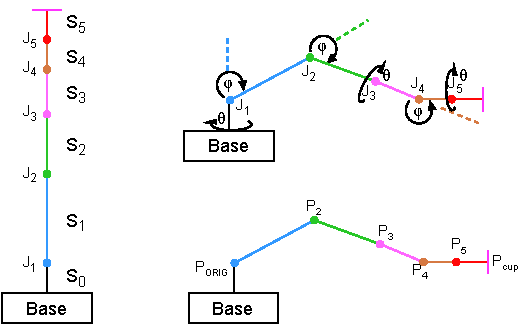
\includegraphics[width=0.9\linewidth, height=6cm,keepaspectratio, center]{Robotic_Arm_segments_Comb.pdf} 
    \caption{Robotic Arm in Segments}
    \label{fig:arm:basestruct}
\end{figure}


The mechanical design and manufacturing of the robotic arm can be found in section \ref{sec:rba:mech}.  This section only focuses on the kinematics of the robotic arm.  

The angle of each joint of the joints of the robotic arm is calculated by using reverse kinematics.  Reverse kinematics refers to finding the position of each motor based on the desired position of the end effector (\sba{pcup}).  $P_i$ is a point in three dimensional space ($[x, y. z]$) for element $i$ in relation to \sba{porig}.  The points $P_4$ and $P_5$ are thus calculated to be perpendicular to the cup at all times, and unless required other wise, calculated to be parallel with the user as well.  This simplifies the calculation of the kinematics as the angle $\theta_{J5}$ is dedicated to keeping the cup upright.

Assume a coordinate system where the x-y plane of the three dimensional space is parallel with the ground and the z-axis is perpendicular to the ground.  The angle $\theta_{J0}$ is calculated based on the desired x and y coordinates of $P_4$ as shown in equation \ref{eq:rba:angj0}.  

\begin{align}
    \theta_{J0} &= \arctan(\frac{Y_{P4}}{X_{P4}}) \label{eq:rba:angj0}
\end{align}

The angle $\varphi_{J2}$ of the joint \sba{j2} can be determined by finding the distance of $P_4$ to \sba{porig}, and using a derivation of Pythagoras' right angle theorem to find the angles inside a triangle when given the lengths of the triangle (equation \ref{eq:rba:innerAng} and figure \ref{fig:rba:triinner}).

\begin{figure}[h]
\centering
    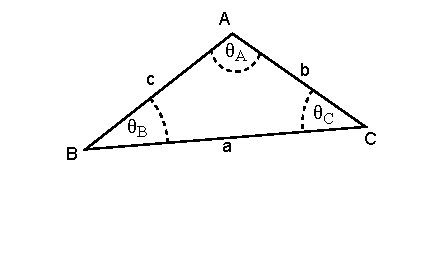
\includegraphics[trim={0 1.8cm 0 0}, width=0.9\linewidth, height=3cm,keepaspectratio, center]{InnerAngl.pdf} 
    \caption{Calculation of the angles of a triangle given the side lengths.}
    \label{fig:rba:triinner}
\end{figure}

\begin{align}
    \theta_A &= \arccos(\frac{b^2+c^2 - a^2}{2bc}) \label{eq:rba:innerAng}
\end{align}

The angle of \sba{j2} and the coordinates of $P_2$ can be calculated by substituting the variables shown in equation \ref{eq:rba:j2calc} in equation \ref{eq:rba:innerAng}.

\begin{align}
    \begin{split}
        A &= P_2\\
        B &= \sie{porig}\\
        a &= r_{S1,S2S3} = \sqrt{X_{P4}^2 + Y_{P4}^2 + Z_{P4}^2}\\
        b &= l_{S2} + l_{S3}\\
        c &= l_{S1}\\
    \theta_A &= 180 - \varphi_{J2}
    \end{split} \label{eq:rba:j2calc}
\end{align}

To calculate the angle of \sba{j1}, the angle $\theta_B$ of the system in equations \ref{fig:rba:triinner} and \ref{eq:rba:j2calc} need to be subtracted off the angle between the Z-axis and $r_{S1,S2S3}$.  The angle between the Z-axis and $r_{S1,S2S3}$ (the angle $\varphi$) can be calculated as shown in figure \ref{fig:rba:polar} and equation \ref{eq:rba:polar2cart}.


\begin{figure}[h]
\centering
    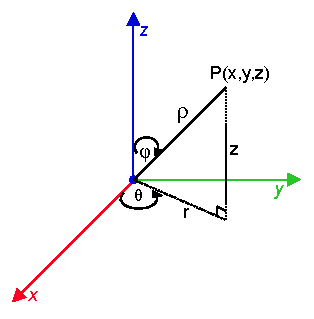
\includegraphics[width=0.9\linewidth, height=5cm,keepaspectratio, center]{cartesian2polar.pdf} 
    \caption{Polar coordinate system.}
    \label{fig:rba:polar}
\end{figure}

\begin{align}
    \begin{split}
        x &=\rho \sin \varphi \cos \theta \\
        y &=\rho \sin \varphi \sin \theta \\
        z &=\rho \cos \varphi
    \end{split} \label{eq:rba:polar2cart}
\end{align}
\begin{align}
    \begin{split}
        \rho^{2} &={x}^{2}+{y}^{2}+z^{2} \\
        \theta &=\arctan\frac{{y}}{{x}} \\
        \varphi &=\arccos \left(\frac{{z}}{\sqrt{{x}^{2}+{y}^{2}+{z}^{2}}}\right)
    \end{split} \label{eq:rba:cart2polar}
\end{align}

Using the angles of \sba{j0} and \sba{j1} and the length of \sba{s1}, the coordinates of the point $P_2$ can be calculated using equation \ref{eq:rba:polar2cart}.  The point $P_3$ in figure \ref{fig:arm:basestruct} can then be calculated as the lengths of \sba{s2} and \sba{s3} are known.  

The angle of the joint \sba{j4} can be calculated by getting the angle between the vectors of the links \sba{s3} and \sba{s4}.  When using the equation \ref{eq:rba:betwvec}, with $\varphi_{vec} = 180-\varphi_{J4}$, the vector of \sba{s3} ($\Vec{\sie{s3}}$) equals vector $\vec{a}$ and the vector of \sba{s4} ($\vec{\sie{s4}}$) equals vector $\vec{b}$.

\begin{align}
    \begin{split}
        \vec{a} &= [x_a, y_a, z_a]\\
        \vec{b} &= [x_b, y_b, z_b]\\
        \rho_a &= \sqrt{x_a^2 + y_a^2 + z_a^2}\\
        \rho_b &= \sqrt{x_b^2 + y_b^2 + z_b^2}\\
        \varphi_{vec} &= \arccos(\frac{x_a\cdot x_b + y_a\cdot y_b + z_a\cdot z_b}{\rho_a\cdot \rho_b})\\
        \varphi_{vec} &= \arccos(\frac{\vec{a}\odot \vec{b}}{\rho_a\cdot \rho_b})
    \end{split} \label{eq:rba:betwvec}
\end{align}

To find $\theta_{J3}$, we first need to define the x and y-axis in the direction of $\vec{\sie{s3}}$.  Using the positions of the robotic arm shown in figure \ref{fig:arm:basestruct} and only focusing on the links \sba{s3} and \sba{s4} (as shown in figure \ref{fig:arm:s3s4}).  We can define the position of the x-axis ($x'_{S3}$) (with all motor angles set to 0\degrs) as shown in figure \ref{fig:arm:s3s4:0pos}.  In a scenario where $\theta_{J0}\neq 0$, the angles of $\theta_{J3}$ and $\varphi_{J4}$ ensure that the links \sba{s4} and \sba{s5} are parallel to the user's position.  The translated and rotated axes of $S3$ (shown in figure \ref{fig:arm:s3s4:use}) can then be used to compute $\theta_{J3}$.  At first the effects of $\theta_{J0}$ are ignored, and 


Using equations \ref{eq:rba:polar2cart} and \ref{eq:rba:cart2polar} a system that can solve for the $\theta_{J3}$ relative to the new axes can be derived, as shown in equation \ref{eq:rba:s3s4}.

\begin{align}
    \begin{split}
        \text{With:}&\\
        z'_{S4} &= l_{S4}\cos(\varphi_{J4})\\
        x'_{S4} &= l_{S4}\sin(\varphi_{J4})\cos(\theta_{J3})\\
        y'_{S4} &= l_{S4}\sin(\varphi_{J4})\sin(\theta_{J3})\\\\
        \text{Substituted into }&\text{equation \ref{eq:rba:cart2polar} gives:}\\
        l_{S4}^2 &= l_{S4}^2\cdot [(\cos\varphi_{J4})^2 + (\sin\varphi_{J4})^2\cdot ((\cos\theta_{J3})^2 + (\sin\theta_{J3})^2)]\\
        \frac{-\cos\varphi_{J4}}{\sin\varphi_{J4}} &= \sqrt{(\cos\theta_{J3})^2 + (\sin\theta_{J3})^2}\\
        -\cot\varphi_{J4} &=
    \end{split} \label{eq:rba:s3s4}
\end{align}

\begin{figure}[h]
    \begin{subfigure}{0.5\textwidth}
        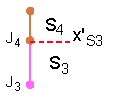
\includegraphics[width=0.9\linewidth, height=4.5cm,keepaspectratio,center]{s3s4_zero.pdf} 
        \caption{$x'_{S3}$ in the primary position of the robotic arm.}
        \label{fig:arm:s3s4:0pos}
    \end{subfigure}
    \begin{subfigure}{0.5\textwidth}
        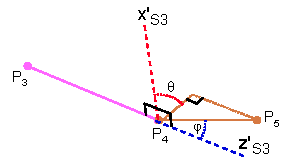
\includegraphics[width=0.9\linewidth, height=4.5cm,center,keepaspectratio]{s3s4Angls.pdf}
        \caption{$x'_{S3}$ and $z'_{S3}$ in a use case.}
        \label{fig:arm:s3s4:use}
    \end{subfigure}
    \caption{Rotated and translated 3D axes of the link \sba{s3}.}
    \label{fig:arm:s3s4}
\end{figure}

\begin{table}[!h]
\centering
\begin{tabular}{|l|l|l|}
\hline
\textbf{Variable} & \textbf{Calculation} & \textbf{Unit} \\ \hline\xrowht[()]{20pt}
$\theta_{J0}$      &  $\arctan(\frac{Y_{P4}}{X_{P4}})$ & degrees    \\\hline\xrowht{20pt}
$r_{S1,S2S3}$     &  $\sqrt{X_{P4}^2 + Y_{P4}^2 + Z_{P4}^2}$   &  mm  \\ \hline\xrowht{20pt}
$\varphi_{J2}$    &  $180 - \arccos(\frac{(l_{S2}+l_{S3})^2+l_{S1}^2 - r_{S1,S2S3}^2}{2\cdot(l_{S2}+l_{S3})\cdot l_{S1}})$    &  degrees             \\ \hline\xrowht{20pt}
$\varphi_{r123}$     &  $\arccos(\frac{Z_{P4}}{r_{S1,S2S3}})$   &  degrees  \\ \hline\xrowht{20pt}
$\varphi_{J1}$     &   $\varphi_{r123} - \arccos(\frac{r_{S1,S2S3}^2+l_{S1}^2 (l_{S2}+l_{S3})^2}{2\cdot r_{S1,S2S3}\cdot l_{S1}})$                   &    degrees           \\ \hline\xrowht{20pt}
\multirow{3}{*}{\centering $P_2$}     & $X_2 = l_{S1}\sin (\varphi_{r123}) \cos (\theta_{J0})$ & \multirow{3}{*}{mm} \\\xrowht{20pt} %\cline{2-2}
                           & $Y_2 = l_{S1}\sin (\varphi_{r123}) \sin (\theta_{J0})$ & \\ \xrowht{20pt}%\cline{2-2}
                           & $Z_2 = l_{S1}\cos (\varphi_{r123})$ & \\\hline \xrowht{20pt}
$\varphi_{J4}$       &  $180-\arccos(\frac{\vec{\sie{s3}}\odot \vec{\sie{s4}}}{l_{S3}\cdot l_{S4}})$                    &    degrees           \\ \hline
\end{tabular}
\caption{Calculation of angles and positions of variables shown in figure \ref{fig:arm:basestruct}.}
\end{table}
%                  &                      &               \\ \hline
%
%
%

\subsubsection{Calculation of Reverse Kinematics}

To calculate the reverse kinematics of the robotic arm the only variable required is the desired position of the end effector relative to \sba{j1}.  This could be the cup's position or the user's mouth.  As no liquid is desired to be spilt from the cup during transport, the links \sba{s4} and \sba{s5} are set so the cup will be kept perpendicular to the ground except when being tilted for the user to drink from the cup.  The 





\rf{Make Table of lengths and rotations}


\subsection{How each corner was calculated}
\subsection{Calibration of potentiometers}
\subsection{Robotic arm design and manufacturing} \label{sec:rba:mech}

As the focus of the final year project is an electronics engineering project, the mechanical design is not discussed in depth and topics such as the material selection, in depth gear and bearing design, the part-by-part assembly of the robotic arm, the in depth manufacturing methods nor the maintenance of the product.

\subsubsection{Force Calculation}



\subsection{Robotic arm control}

\section{Cup}
\subsection{capacitive liquid level sensing}
\subsection{Accelerometer/Gyroscope calibration}
\subsection{system meshing}



\glsaddall
% ________________________________________________
%                   Glosseries
% ________________________________________________
\renewcommand{\arraystretch}{1.5}
\newglossarystyle{symbunitlong}{%
\setglossarystyle{long3col}% base this style on the list style
\renewenvironment{theglossary}{% Change the table type --> 3 columns
  \begin{longtable}{lp{0.6\glsdescwidth}>{\centering}p{2cm}>{\centering\arraybackslash}p{2cm}}}%
  {\end{longtable}}%
  
%
\renewcommand*{\glossaryheader}{%  Change the table header
  \bfseries Symbol & \bfseries Description & \bfseries Unit & \bfseries Equation\\
  \hline
  \endhead}


\renewcommand*{\glossentry}[2]{%  Change the displayed items
\glstarget{##1}{\glossentryname{##1}} %
& \glossentrydesc{##1}% Description
& \glsunit{##1} 
& \glseqn{##1} \tabularnewline
}
}

\newpage
% \printglossary[type=symbolslist,style=symbunitlong,title={Symbols}]   % list of symbols
\printnoidxglossary[type=symbolslist,sort=use,style=symbunitlong,title={Symbols}]
\newpage
\printglossary[type=main]
\newpage
\printglossary[type=\acronymtype]





\section{Appendix 4: Code}

\subsection{Facial Recognition}

\subsubsection{Viola Jones}
% \textbf{Integral image calculations}
% \pyCode{ViolaJones/integralImaging.py}
\pyCode{ViolaJones/fullViolaJonesTraining.py}

\mlCode{harris.m}


\end{document}
